%%O+I
%% Dominic
%%24 Dec 2004 => final

\ifx\wholebook\relax\else
\input{../Common.tex}
\input{../macroes.tex}
\begin{document}
\fi

\newcommand{\dist}[0]{middle\xspace}


\chapter{Variables}\label{ch:variables}\label{cha:variable}\label{cha:variables}

\begin{chapterfigure}
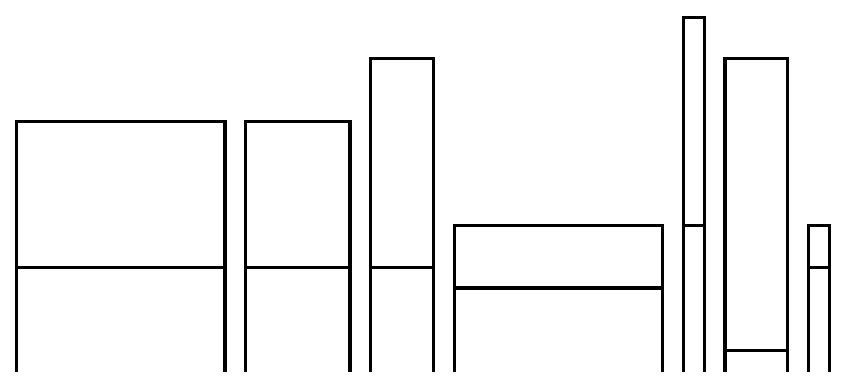
\includegraphics[width=0.9\linewidth]{varTitlePicture}
\end{chapterfigure}

\hidden{|\caro |
	\caro := \Turtle new.
	\caro west.
	\caro jump: 300.
	\caro varALetterHeight: 120 width: 100 middle: 50.
	\caro east.
	
	\caro jump: 10.
	\caro varALetterHeight: 120 width: 50 middle: 50.
	\caro east.
	
	\caro jump: 10.
	\caro varALetterHeight: 150 width: 30 middle: 50.
	\caro east.

	\caro jump: 10.
	\caro varALetterHeight: 70 width: 100 middle: 40.
	\caro east.
	
	\caro jump: 10.
	\caro varALetterHeight: 170 width: 10 middle: 70.
	\caro east.

	\caro jump: 10.
	\caro varALetterHeight: 150 width: 30 middle: 10.
	\caro east.

	\caro jump: 10.
	\caro varALetterHeight: 70 width: 10 middle: 50.


varALetterHeight: height width: width middle: middle


	self north.
	self go: height.
	self east.
	self go: width.
	self south.
	self go: height.

	self west.
	self jump: width.
	self north.
	self go: middle.
	
	self east.
	self go: width.
	self south.
	self go: middle.

}


We are constantly giving names to human beings or things. For example,
we give names to people, to dogs or to cars. By doing that we are
\strong{associating} something to a word or a symbol. Once this association is done,  we then later use the word or symbol to \strong{refer to} or to interact
with the thing associated with it. Sometimes, names are for a lifetime
or sometimes just for a short period of time. Sometimes names
refer to other names. For example, an actor has several names, a
public name, a civil name and a name of the character he is playing in
a movie.  In a programming language, we also need to be able to name things and variables are used for that. 

In this chapter, we introduce \strong{variables} which are placeholders for objects and show how variables help to simplify programs. Moreover using variables is sometimes necessary for programming. Finally, as the complexity of problems you will facing will  increase, you will see that you will need to express dependencies between variables. For example, the width of a rectangle can be 2/3 of its length. In this chapter we show how to use variables to express dependencies between numbers.



\section{A World of As}
As asked in Chapter~\ref{ch:TurtleMen}, suppose that we want to use a
robot to write letters. The character A is characterized by a
\strong{height}, a \strong{width} and a \strong{\dist} from which the middle line of the A should be drawn as shown by Figure~\ref{exo:a100}.

\begin{exofigwithsize}{\includegraphics[width=4cm]{varAnnotated}}\label{exo:a100}
Propose a script that draws a character A of 100 pixel height, 70
pixel width and 60 pixel \dist (distance between the ground and the first horizontal line).
\end{exofigwithsize}


\paragraph{Variations on A.}
The script you wrote for answering the \exoref{exo:a100} should look
somehow like the following script \ref{src:a100}.

\begin{scriptwithtitle}{An A of 100}\label{src:a100}
| \caro |
\caro := \Turtle new.
\caro north.
\caro go: 100.
\caro east.
\caro go: 70.
\caro south.
\caro go: 100.
\caro west.
\caro jump: 70.
\caro north.
\caro go: 60.
\caro east.
\caro go: 70
\end{scriptwithtitle}

\begin{exofigwithsizeandtitle}[0.5]{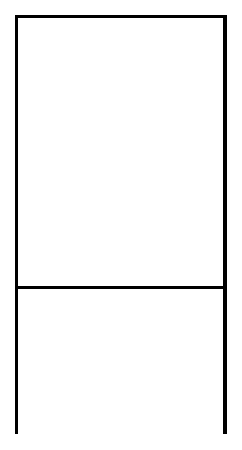
\includegraphics[width=1.5cm]{varA200}}{frAnkenstein}\label{exo:a200}
Change the \scriptref{src:a100} to draw an A of 200 pixel height, 100
pixel width and 70 pixel \dist.
\end{exofigwithsizeandtitle}


As the previous experiment \ref{exo:a200} shows you, every times we want to produce an A of a different size we have to change \strong{everywhere} and
\strong{synchronously} the numbers that represent the height, the
width and the \dist of the letter. By synchronously, we mean that 100 should become
200, 70 should become 100 and 60 should become 70 without mixing them.

\begin{exonofig}
Change the \scriptref{src:a100} to draw other A letters with different
sizes of your choice.  Try to reproduce some of the As that compose the opening
picture of this chapter.
\end{exonofig}


As you may notice, having to change the values everywhere is
tedious. Moreover, you also may risk becoming confused and forget to
change a value at one place.  This can  result in breaking the
script. You can easily imagine that in complex programs this is
a real problem to change values in such a way.

\section{Variables to the Rescue}
As seen with the previous exercises producing letters of different
size can be tiresome and errorprone as you can mixed the number representing the various lengths of a letter. We have to take care to change all the values everywhere. In fact, we would like to be able to:

\begin{itemize}
\item \strong{declare} the height, width and \dist of an A once for all, 
\item being able to \strong{refer to} these values, and 
\item possibly \strong{change} the values if necessary. 
\end{itemize}

This is exactly what a variable allows us to do! Amazing isn't it? A variable is a \strong{name} to which we \strong{associate a value}. We must \emph{declare} it and  \emph{associate} a new value to it. Then we can \strong{refer to} a variable and obtain the \emph{value} associated with this variable. It is also possible to \strong{modify} the value associated with a variable and associate it a new value. The variable value can be a number, a collection of objects, ... even a robot. We now illustrate how to declare, associate a value and use a variable.

\largecadre{
A variable is a \strong{name} to which we \strong{associate a value}. We \emph{declare} a variable and  \emph{associate} a value to it. Then we can \strong{refer to} a variable and obtain its \emph{value}. It is also possible to \strong{modify} the value associated with a variable and associate a new value to it.}

\subsection*{Declaring a variable}
Before using a variable, we have to \strong{declare} it, that is telling to the system the name of the variable that we want to use. We declare variables by enclosing them with vertical bars \ct{||} as shown by the following example which declares three variables \ct{height}, \ct{width} and \ct{\dist}.  To be exact, vertical bars \ct{||} declare temporary variables \ie variables that only exist during the execution of the script.

\begin{nalltt}
| height width middle |
\end{nalltt}



\subsection*{Assigning a value to a variable}
Before using a variable it is better to give it a value. Associating a value is called \strong{assigning} a value to a variable. In \st, \ct{:=} is used to assign a value to a variable. In the following script after declaring the three variables we assign 100 to 
the variable \ct{height}, 70 to the variable \ct{width} and 60 to the variable \ct{\dist}.
When this is the first time that we assign a value to a variable, we say that we \strong{initialize} it.

\begin{nalltt}
| height width middle |
height := 100.
width := 70.
\dist := 60
\end{nalltt}

\largecadre{\ct{:=} assigns a value to a variable. Example: \ct{height := 120} assigns the  \ct{120} to the variable \ct{height}.  \ct{length := 120 + 30} assigns the result of the expression  \ct{120 + 30} \ie \ct{150} to the variable \ct{length}.} 

\largecadre{When this is the first time that we assign a value to a variable we say that we initialize it.}

\subsection*{Referring to Variables}
To refer to the value assigned to a variable \--- we also say use a variable, you simply write its name in a script. In the following script, after being declared line 1, the variable \ct{height} is initialized  with the value 100 in line 2 and used line 4 to say to the created robot to go forward from the \ct{height}  variable's value, here 100.

\begin{nalltt}
| \caro height |
\caro := \Turtle new.
height := 100
\caro north.
\caro go: \textbf{height}
\end{nalltt}


\largecadre{Generally a variable must be \strong{declared} and \strong{initialized}, before being used.}


\subsection*{About \caro}
Yes, you guessed right! \caro is also a variable, just a variable whose value is a robot. Hence, \ct{| \caro |} declares that you use a variable named \ct{\caro}. The expression \ct{\caro\ := \Turtle new} initializes the variable with a value, here a new robot. Then we use this robot by sending messages to it via the variable \ct{\caro}, for example \ct{\caro go: 100.}

\section{Using Variables}
Now let us explore the benefits of using variables and show you some powerful properties. In particular, we show that been able to express relationships between variables is really powerful.  

Once we introduce variables in the \scriptref{src:a100}, we obtain the
\scriptref{src:a100var}.

\begin{scriptwithtitle}{An A of 100}\label{src:a100var}
| \caro \textbf{height width \dist}|
\caro := \Turtle new.
\textbf{height := 100.}                       "initializes the variables"
\textbf{width := 70.}
\textbf{\dist := 60.}
\caro north.
\caro go: \textbf{height.}                    "then we use the variables"
\caro east.
\caro go: \textbf{width.}
\caro south.
\caro go: \textbf{height.}
\caro west.
\caro jump: \textbf{width.}
\caro north.
\caro go: \textbf{\dist.}
\caro east.
\caro go: \textbf{width}
\end{scriptwithtitle}

Now changing variable values is easier. Change some values to convince yourself. You should be able to draw all the As that are drawn in the first picture of this chapter.
Now to produce a new letter with different lengths you \emph{just} have to change their values during their initialization as shown in script~\ref{src:b100var} and whose result is presented in Figure~\ref{fig:varAFlat}.

\begin{scriptwithtitle}{An A of 100}\label{src:b100var}
| \caro \textbf{height width \dist}|
\caro := \Turtle new.
\textbf{height := 30}.                "initializes the variables"
\textbf{width := 200}.
\textbf{\dist := 10}.
...
\end{scriptwithtitle}

\begin{figure}[h]
\begin{center}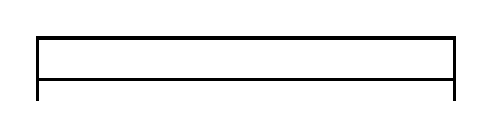
\includegraphics{varAFlat}\end{center}
\caption{A flat A letter simply created with \textbf{height = 30}, \textbf{width = 200}, and 
\textbf{\dist = 10}.}\label{fig:varAFlat}
\end{figure}

Using variables you can easily create a lot a different characters and solve a lot of problems in the future. It is now worth to step back and look at the power provided by variables.

\paragraph{Analysing the Power of Variables.}
These experiments illustrate the power of using variables. Variables let you name a thing, being a robot, a length, or anything else.  Then you can use these names instead of repeating the values that you associated with the variables. Using variables make your scripts more easy to change as you can simply change the variable values. In addition a variable can be holding any kind of values: up until now you assigned robots or numbers to variables but it could be a color (for example \ct{yellowCol := Color yellow}), a sound or any \sq objects. 

Note also that by using variables your scripts are much more readable and easier to understand. To convince yourself just compare the scripts~\ref{src:a100} and \ref{src:a100var}.  The simple fact of using variables with names such as ``width'' and ``height'' helps you to understand how the letter is drawn. 

\subsection{Expressing Relationships between Variables}
The characters in a font should respect certain proportions to ease reading, that is the lengths that describe a character are not freely chosen but maintain certain proportions between them. 

In our simple character A, let us decide that the width should be 2/3 of the height and that the \dist should be at 3/5 of the height. We can express these relationships using variables as shown in the following \scriptref{src:a100varl}. Indeed the value of a variable does not have to be  limited to a simple number but can be the result of a complex computation. 

\begin{scriptwithtitle}{Towards a Solution}\label{src:a100varl}
| \caro height width \dist|
\caro := \Turtle new.
height := \textbf{120}.
width := \textbf{120} * 2 / 3.
\dist := \textbf{120} * 3 / 5.
...
\end{scriptwithtitle}

If you analyze a bit the \scriptref{src:a100varl}, you realize that it is not optimal. The relationships are expressed between the variables, but still the value 120 (in lines 3,4 and 5) has to be changed manually when we want to produce a different A holding the same relations.  The solution is to use the variable \ct{height} instead of \ct{120} as shown in \scriptref{src:a100varwl}. In this script, the value of the variables \ct{width} and \ct{\dist} depends on the one of \ct{height}. The value of a variable can be expressed by using other variables. The expression \ct{width := height * 2 / 3} expresses that the width of the character is equal to 2/3 of the height.

\begin{scriptwithtitle}{Making \ct{width} and \ct{\dist} depending on \ct{height}}\label{src:a100varwl}
| \caro height width \dist|
\caro := \Turtle new.
\textbf{height := 120}.
width := \textbf{height} * 2 / 3.
\dist := \textbf{height} * 3 / 5.
\caro north.
...
\end{scriptwithtitle}


\paragraph{Important.} The only constraint we have while expressing relationships between variables is that the value of variable used in the definition of
another should be known. For example, in \scriptref{src:a100varwl},
the value of \ct{height} is known while computing the value of
\ct{width} and \ct{\dist}.  On the contrary, in \scriptref{src:wrong} the value of \ct{height} is not known when the value of \ct{width} is computed, this leads to an error. We will elaborate more on errors in Chapter~\ref{ch:debugger}.

\begin{scriptwithtitle}{Problematic \ct{width} initialization}\label{src:wrong}
| height width \dist |
width := height * 2 / 3.
height := 120.
\dist := height * 3 / 5.
\end{scriptwithtitle}

Now you see that variables are really useful to express complex relationships and can hold any kind of objects.

\section{Some Experimentations}
We recommend you gain some experience with the following problems.

\begin{exofigwithsizeandtitle}[.8]{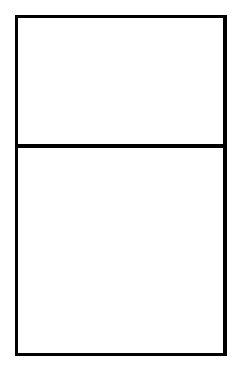
\includegraphics[width=2.5cm]{varGoldenRec}}{Golden Rectangle}\label{exo:goldenrectangle}

A golden rectangle is a rectangle whose height is 1.6 times its width
--- 1.6 is an approximation of the golden number $\frac{1 +
\sqrt{5}}{2}$ which is the side of a regular decagon inside a circle
of unity.  The nice property of such a rectangle is that if we draw
inside the rectangle a square with size the rectangle's width, then
the left part of the rectangle is again a golden rectangle. Such a
property is then infinite. Ancient architects were using a lot such a golden proportion in their constructions. Every rectangle created this way is a
golden rectangle. Define a script that draws a golden rectangle.
$\frac{1 + \sqrt{5}}{2}$ is expressed in Smalltalk as \ct{1 + 5 sqrt /
2}.

\end{exofigwithsizeandtitle}


\hidden{
| \caro height width|
\caro := \Turtle new.
width := 100.
height := width * ((1 + 5 sqrt)/2).
\caro go: width.
\caro turnLeft: 90.
\caro go: height.
\caro turnLeft: 90.
\caro go: width.
\caro turnLeft: 90.
\caro go: height.
\caro turnLeft: 90.
\caro go: width.
\caro turnLeft: 90.
\caro go: width.
\caro turnLeft: 90.
\caro go: width
}

\begin{exonofig}
Explain why none of the following scripts do not draw an A of 120
pixel height.
\begin{nalltt}
\begin{tabbing}
aaaaaaaaaaaaaaaaaaaaaaaaaa\=aaaaaaaaaaaaaaaaaaaaaaaaaa\kill
| \caro height |               \>| \caro height |       \\             
\caro := \Turtle new.         \>\caro := \Turtle new.\\
height := 120.                   \>\caro north.\\
\caro north.                      \>\caro go: height.\\
\caro go: 100.                      \>\caro east.\\
\caro east.                               \>\caro go: 70.\\
\caro go: 70.                               \>\caro south.\\
\caro south.                              \>\caro go: height.\\
\caro go: 100.                             \>\caro west.\\
\caro west.                                 \>\caro jump: 70.\\
\caro jump: 70.                            \>\caro north.\\
\caro north.                                  \>\caro jump: 50.\\
\caro jump: 50.                              \>\caro east.\\
\caro east.                                       \>\caro go: 70\\
\caro go: 70
\end{tabbing}
\end{nalltt}
\end{exonofig}

\paragraph{Pyramids rediscovered.} In Section~\ref{sec:bouclonpyramids} of Chapter~\ref{ch:looping} in the \scriptref{scr:pyramid} 
we defined the outline of the pyramid of Saqqarah the following way.

\begin{scriptfigwithsize}[.45]{\includegraphics[width=8cm]{varPyramid}}{Pyramid script}
| \caro |
\caro := \Turtle new.
5 timesRepeat: 
               [ \caro north.
               \caro go: 20.
               \caro east.
               \caro go: 20 ].
5 timesRepeat: 
               [ \caro go: 20.
               \caro south.
               \caro go: 20.
               \caro east ].
\caro west.
\caro go: 200.
\end{scriptfigwithsize}


\begin{exonofig}
Introduce the variable \ct{terracesNumber} that represents the
 number of terraces that the pyramid can have. 
\end{exonofig}

\begin{exonofig}
In the previous script introduce the variable \ct{terraceSize} that represents the size of a terrace.
\end{exonofig}
 
\section{Another Example of Variable Use}
The use of variables greatly simplifies the definition of scripts where some of the \emph{variables} depend on other ones. In this section, we shall see how the use of variables gives great leverage when dealing with loops. The Chapter~\ref{ch:loopvar} will go deeper in showing that the combination of variables and loops is powerful.

Let us look again for a moment at the experiements~\ref{exo:pentagonRepeat} and
\ref{exo:hexagonRepeat} in which a \Turtle was asked to draw a
pentagon and a hexagon. 

\begin{scriptfigwithsize}[.5]{\includegraphics[width=4.5cm]{varFPentagon}}{Pentagon}
| \caro |
\caro := \Turtle new.
5 timesRepeat: 
               [ \caro go: 100.
               \caro turnLeft: 72 ]
\end{scriptfigwithsize}

\begin{scriptfigwithsize}[.5]{\includegraphics[width=4.5cm]{varFHexagon}}{Hexagon}
| \caro |
\caro := \Turtle new.
6 timesRepeat: 
               [ \caro go: 100.
               \caro turnLeft: 60 ]
\end{scriptfigwithsize}

The difference between the two scripts is that one must change the
number of sides (let us call it $s$) \emph{and} the magnitude of the
turn (let us call it $T$) such that the product $s\times T$ is equal
to 360. Wouldn't it be nice if we could write a script, in which we
only would have to change a single number, let us say the number of
sides since this is the easiest parameter to choose?  This is possible
by introducing variables. Try to come up with your own solution.  




Here is a script where this is done (Script~\ref{scr:regularPolygon}). Try it
before we discuss more about it. 

\begin{scriptwithtitle}{Regular polygon}\label{scr:regularPolygon}
| \caro sides angle |
\caro := \Turtle new.
sides := 6.
angle := 360 / sides.
sides timesRepeat: 
                  [ \caro go: 100.
                  \caro turnLeft: angle ]
\end{scriptwithtitle}

We have introduced two new
variables --- \ct{sides} and \ct{angle} --- used to hold
the needed values. Then, the line \ct{sides := 6} assigns the
value 6 to the variable \ct{sides} and the line \ct{angle
:= 360 / sides} assigns a value to the variable angle, which is
the result of 360 divided by the value held in the variable
\ct{number}. The value of the variable \ct{angle} is then
used as argument of the command \turnLeft given to
the robot in the repeating block.


\section{Regular Polygons with Fixed Sizes}

If you have used Script~\ref{scr:regularPolygon} with a large number of sides, you will have noticed that the resulting figure did not fit on the screen.  The next exercise asks you to fix this by reducing the
length of the sides when the number of sides augments.

\begin{exofig}{varSameLength} \label{exo:fixedSizePolygon}
Modify Script~\ref{scr:regularPolygon} so that the size of the
regular polygon stays constant as the number of sides changes.

Hint: introduce a variable length which is set to a fixed length
divided by the number of sides.
\end{exofig}

\hidden{| \caro sides angle l |
	\caro := \Turtle new.
	sides := 15.
	angle := 360 / sides.
	l := 300 / sides.
	sides timesRepeat: [ \caro go: l.
                  \caro turnLeft: angle ]}

\summa

\begin{enumerate}
\item A variable is a \strong{name} to which we \strong{associate a value}. We must \emph{declare} it and  \emph{associate} a value to it. Then we can \strong{refer to} a variable and obtain the \emph{value} associated with this variable. It is also possible to \strong{modify} the value associated with a variable and associate a new value to it. 
 
\item A variable can be used at any place where its value can be used.  

\item When this is the first time that we assign a value to a variable, we say that we \strong{initialize} it. 

\item \ct{:=} assigns a value to a variable. Example: \ct{height := 120} assigns the  \ct{120} to the variable \ct{height}.  \ct{length := 120 + 30} assigns the result of the expression  \ct{120 + 30} \ie \ct{150} to the variable \ct{length}.

\item A variable must be \strong{declared} and \strong{initialized}, before being used.

\end{enumerate}


\begin{table}[h]
  \centering
\begin{tabular}{| p{5cm} | p{4cm} | l |} \hline
  \hfil Expressions & \hfil Description & \hfil Example \\[1ex] \hline
  \ct{| $\langle$variable name$\rangle$ |} & Declaration of a variable & \ct{| \caro height |}\\ \hline
  \ct{$\langle$length$\rangle$ := $\langle$ \emph{expression} $\rangle$} & Assigns the  value of expression to a variable & \ct{length\ :=\ 40}\\
  && \ct{length := 30 + 20}\\ \hline
  &Uses a variable's value& \ct{\caro go: length}\\ \hline

  &Uses and changes the value of a variable& \ct{length := length + 10}\\
  \hline
\end{tabular}
\end{table}


\ifx\wholebook\relax\else\end{document}\fi
